\documentclass[UTF8]{csoarticle}


\newtheorem{theorem}{定理}
\newtheorem{lemma}{引理}
\renewcommand{\proofname}{证明}
% 如果为英文文章,可以使用下面的定义(去除行首的注释符号%)代替上述中文定义
% \newtheorem{theorem}{Theorem}
% \newtheorem{lemma}{Lemma}

\begin{document}

%----------------------------------------------------------
% 1. 文章标头信息
%----------------------------------------------------------

\titleCHN{基于局部特征的图像重建算法}
\titleENG{Image Reconstruction Based on Local Features}
\authorCHN{王继哲\affil{1},李学明\affil{2}}
\authorENG{WANG Ji-Zhe\affil{1}, LI Xue-Ming\affil{2}}
\affiliationCHN{
    \affil{1} 北京邮电大学信息与通信工程学院,北京 100876 \\
    \affil{2} 北京邮电大学信息与通信工程学院,北京 100876
}
\affiliationENG{
    \affil{1} School of Information and Communication Engineering, Beijing University of Posts and Telecommunications, Beijing 100876 \\
    \affil{2} School of Information and Communication Engineering, Beijing University of Posts and Telecommunications, Beijing 100876
}

\abstractCHN{综述文章:以背景、研究现状、研究用途的结构书写,篇幅以150~300字左右为宜,不用第一人称做主语,不与正文语句重复。一般研究性文章:以摘录要点的形式按目的、方法、结果、结论的结构报道出作者的主要研究成果,字数在200~400字左右为宜,不用第一人称做主语,不与正文语句重复。
基于局部特征的图像重建算法是利用原始图像的局部特征信息,以大图像集为数据源,进行较为精确的图像重建工作,使重建后的图像与原始图像相似,并且图像质量达到人眼主观效果较好的程度。本文首先对目前图像重建算法加以概述,综合介绍重建系统中的局部特征、视觉词组、相似图像搜索、特征匹配、特征配准、匹配特征块筛选、图像融合等多种计算机视觉相关技术。之后将该系统引入大语料集的应用场景下,对上述几个环节进行完善,主要包括在(1)相似搜索环节引入GEO-Hash索引技术并提出分块相似搜索,一方面极大加快了搜索速度,另一方面提高了搜索结果的多样性;(2)在匹配块筛选法中提出阈值自适应的验证准则。为匹配块的筛选提供更有力的依据,显著提升了拼接结果。}

\abstractENG{abstract text}
\keywordCHN{中文关键词要能反映文章的基本观点,避免广义词。第一个关键词为该文内容所属二级学科名称}
\keywordENG{list of keywords}
\cateidCHN{请查阅《中国图书馆分类法》}

\authorIntroduction{王继哲(1989-),男,硕士研究生,主要研究方向:多媒体通信,图像处理。通信作者:李学明(1969-),男,教授,主要研究方向:多媒体通信,图像处理。}
\fund{***基金(00000000),***基金(00000000)}

\maketitle


%----------------------------------------------------------
% 2. 正文内容
%----------------------------------------------------------

\section{引言}

简要回顾研究工作的背景和研究目的,一般400~600字,不超过800字。

随着移动终端计算能力的提升,终端应用迎来蓬勃发展,图片类应用日益普及,每天有数以万计的高分辨率图像由移动终端上传到服务器上,给通信网络带宽造成了巨大的压力。
另一方面我们观察到随着存储设备容量变大、芯片计算能力的提升,互联网用户的不断增多,大数据时代来临。图像数据数以亿计,服务器计算能力极大提升。从信息的角度来说,我们拍摄的每一幅图像中所包含的部分或全部内容都可以在互联网上其它图像中找到。

在2013年有学者[文献6]提出一种全新的压缩方式——基于云的图像编码。其核心思想是在客户端提取并编码发送少量的图像特征数据,并不传输图像数据本身,而在服务器端解码后利用特征数据在服务器的大图像数据集上匹配相似的图像,利用相似图像进行图像的重建。这种架构所运用的核心技术手段便是基于局部特征的图像重建算法。系统的核心思想是通过对原始图像的特征提取与重建,利用计算资源减少带宽损耗,从一个全新的维度进行数据压缩,为多媒体应用开启了一扇大门。

图像重建任务的核心是通过局部特征找到与原始图像相似的图像单元以及可靠的图像间对应点集合,进而自动地建立图像之间点与点或区域与区域之间的可靠对应关系,根据对应关系采用一定的算法拼接图像单元。基于局部特征对图像进行重建的技术能够让我们在发送端只传输少量的特征数据,而接收端服务器利用大数据集进行高分辨率图像的还原。

本文在上述的大框架下综合使用多种信息检索与图像处理技术,对其中的相似图像检索、图像块筛选等核心算法进行了改进与完善,使之更加能够适用于大规模图像集上的图像重建任务,重建速度得到提升,重建结果得到了进一步的优化。

\section{基于局部特征的图像重建算法}
在本文的应用场景下,图像重建的部分流程可以看成是多幅图像的全景图拼接问题。与文献\cite{Brown:2006ir}中的流程类似,主要包含以下几个环节:(1)使用具有不变性的特征来描述图像;(2)自动的找到图像之间的空间位置关系,进行图像配准;(3)图像融合,消除不同图像之间的光照差别,去除边缘噪声。与全景图拼接不同的是,本文的图像重建系统以图像块(Patch)和下采样图像为输入,如何解决图像块大小不一空间位置以及像素值准确度低的问题,如何充分利用下采样图像信息优化图像融合是本文尝试解决的问题,现分别介绍如下。

\subsection{图像的局部特征}
图像的局部特征是计算机视觉领域一个基本问题,它能够反映图像某一局部的特性,对寻找图像对应的局部单元以及特征描述中有着重要作用。描述的核心问题是不变性和可区分性。

在多种局部特征中,本文选择使用Lowe提出的尺度不变特征变换(Scale Invariant Feature Transform,以下简称SIFT)。SIFT算子是图像局部特征研究领域的一项重大突破。SIFT算子具有很强的可区分性,同时对尺度、旋转以及一定视角和光照变化等图像变化都具有不变性。

\subsubsection{尺度空间理论}
尺度空间是模拟图像数据的多尺度特征:尺度空间中图像的模糊程度逐渐变大,能够模拟人在距离目标由近到远时目标在视网膜上的成像过程。我们可以把两幅图像想象成是连续的,分别以它们作为底面作四棱锥,就像金字塔,那么每一个截面与原图像相似,金字塔的两层中包含无穷个截面,在实际应用只能选择离散诘责,构造有限个层。

\subsubsection{SIFT检测子与描述子}
SIFT算法有两个主要环节,一个是检测“感兴趣”的关键点,另一个是描述这个“关键点”。SIFT关键点是精心选择的一组在高斯差分尺度空间上的极值点,该关键点包含三个关键信息,分别是(1)亚像素精度的(x,y)位置信息;(2)尺度大小,反映关键点局部的大小,同时决定了特征的覆盖范围,对后文局部块的提取起到至关重要的作用;(3)所在高斯尺度空间上的主方向,该主方向是有一个高斯窗口函数计算得来,反映的是关键点所在局部的方向信息。

SIFT描述子反映关键点局部的信息,是高斯尺度空间上某一局部和方向上的梯度信息,以直方图的形式对信息做统计,最终每一个描述子是一个128的特征。

\subsection{特征匹配}
当我们通过相似图像搜索获得与原图近似的图像后,需要精确的找到原始图像与候选拼接图像相匹配的特征点,其匹配策略为:
\begin{equation}
  M(S_1,S_2) = 
\begin{cases} 
\text{true}, & \mbox{if } S_2 = S_{min},\frac{\text{Dis}(S,S_{min})}{\text{Dis}(S,\tilde{S}_{min})} > C \\
\text{false}, & \mbox{otherwise}
\end{cases}
\end{equation}
其中\(\text{Dis}(\cdot,\cdot)\)表示的是两个特征描述子之间的相似性度量,比如可以用欧氏距离表示,距离越大,相似性越小。\(S_{min}\)和\(\tilde{S}_{min}\)分别表示的是与S距离最近和第二近的特征。而C是一个阈值常数,通常取1.5。

匹配通常采用k-d树\cite{李航2012统计学习方法}技术进行最近邻搜索。对于n个实例的k维数据来说,建立kd-tree的时间复杂度为O(k*n*logn)。时间复杂度比暴力法要降低很多。

\subsection{图像配准}
匹配完成后,原始图像的SIFT特征\(S\)匹配到了候选图像中的特征\(\tilde{S}\),通过匹配的特征对我们可以得到两个对应的图像块,原图图像块\(P_S\)和候选图像块\(P_\tilde{S}\),图像块是根据SIFT特征\((x_f,y_f,s_f,\theta))\)以及对应的图像得到的。本文选取的是正方形图像块,其中尺度决定了图像块的大小。

当一个图像块中的多个SIFT特征匹配之后,我们找到了多个匹配的图像块,这时每对图像块都是正方形构成,我们希望对候选图像块做进一步的投影变换,使之与源图像块更为精准的匹配,这一环节叫做图像配准。

根据文献\ref{},有两种配准方式,一种是直接写出变换矩阵,另一种是使用RANSAC方式多次迭代找到最准确的变换矩阵。RANSAC的方式将在后文介绍,我们先介绍根据一对匹配的SIFT算子直接写出两个图像块的变换矩阵。

结合一对匹配SIFT特征点\(\tilde{S}\)和\(S\)的位置、尺度和方向,我们可以得到两个图像块\(P_{\tilde{S}}\)和\(P_S\)的变换矩阵\(H_0\):

\begin{equation}
  H_0 = 
  \begin{bmatrix}
  \frac{\tilde{s}_f}{s_f} R & T
  \end{bmatrix}
\end{equation}
其中
\begin{equation}
  R = 
  \begin{bmatrix}
    \cos{(\tilde{\theta}-\theta)} & -\sin{(\tilde{\theta}-\theta)} \\
    \sin{(\tilde{\theta}-\theta)} & \cos{(\tilde{\theta}-\theta)} 
  \end{bmatrix}
\end{equation}

\begin{equation}
  T = 
  \begin{bmatrix}
    \tilde{x}_f - x_f \\
    \tilde{y}_f - y_f
  \end{bmatrix}
\end{equation}

计算出的\(H_0\)和\(H\)都可以作为块的旋转矩阵,在实际的系统中,我们会同时计算两个矩阵,比较他们的准确程度,挑选使用准确度高的变换矩阵,在实验中,因为我们采用下采样图像的均方误差做验证,而下采样图像本身的精度损失导致误差估计不准确,所以我们采用如下的策略:当匹配块内匹配特征点多时,我们更倾向于使用RANSAC算法计算得到的变换矩阵,反之我们更倾向于使用直接计算法。

\subsection{自适应图像块筛选法}
图像重建任务的最后一个步骤是图像融合,在此之前我们已经得到了每个源图像特征对应的候选图像块,图像块的方向、尺度、位置都有所不同,图像块之间可能存在交叠,部分图像块与原图存在较大误差,需要利用下采样图像计算配准后的图像块与源图像块的误差,根据设定好的阈值\(\epsilon\)移除误差较大的图像块。

在文献\ref{}中作者提到使用对上述配准后的图像块使用基于图的图像分割方案,对每一个分割连通域做均方误差校验,相当于图像块做进一步的细分,能够有效去除图像块中不匹配的部分。在实际测试中,由于我们在高分辨率图像重建场景下,导致图像分割与图像像素数量成正比,资源消耗过大,另一方面分割导致图像粒度过细,验证步骤的误差存在难以保证筛选结果的准确,因此我们在此省略了精细化分图像块的步骤,提出了一种自适应阈值的图像块筛选法。

服务器端在线重建如图\ref{fig:serverOnline}所示:
\begin{figure}
\centering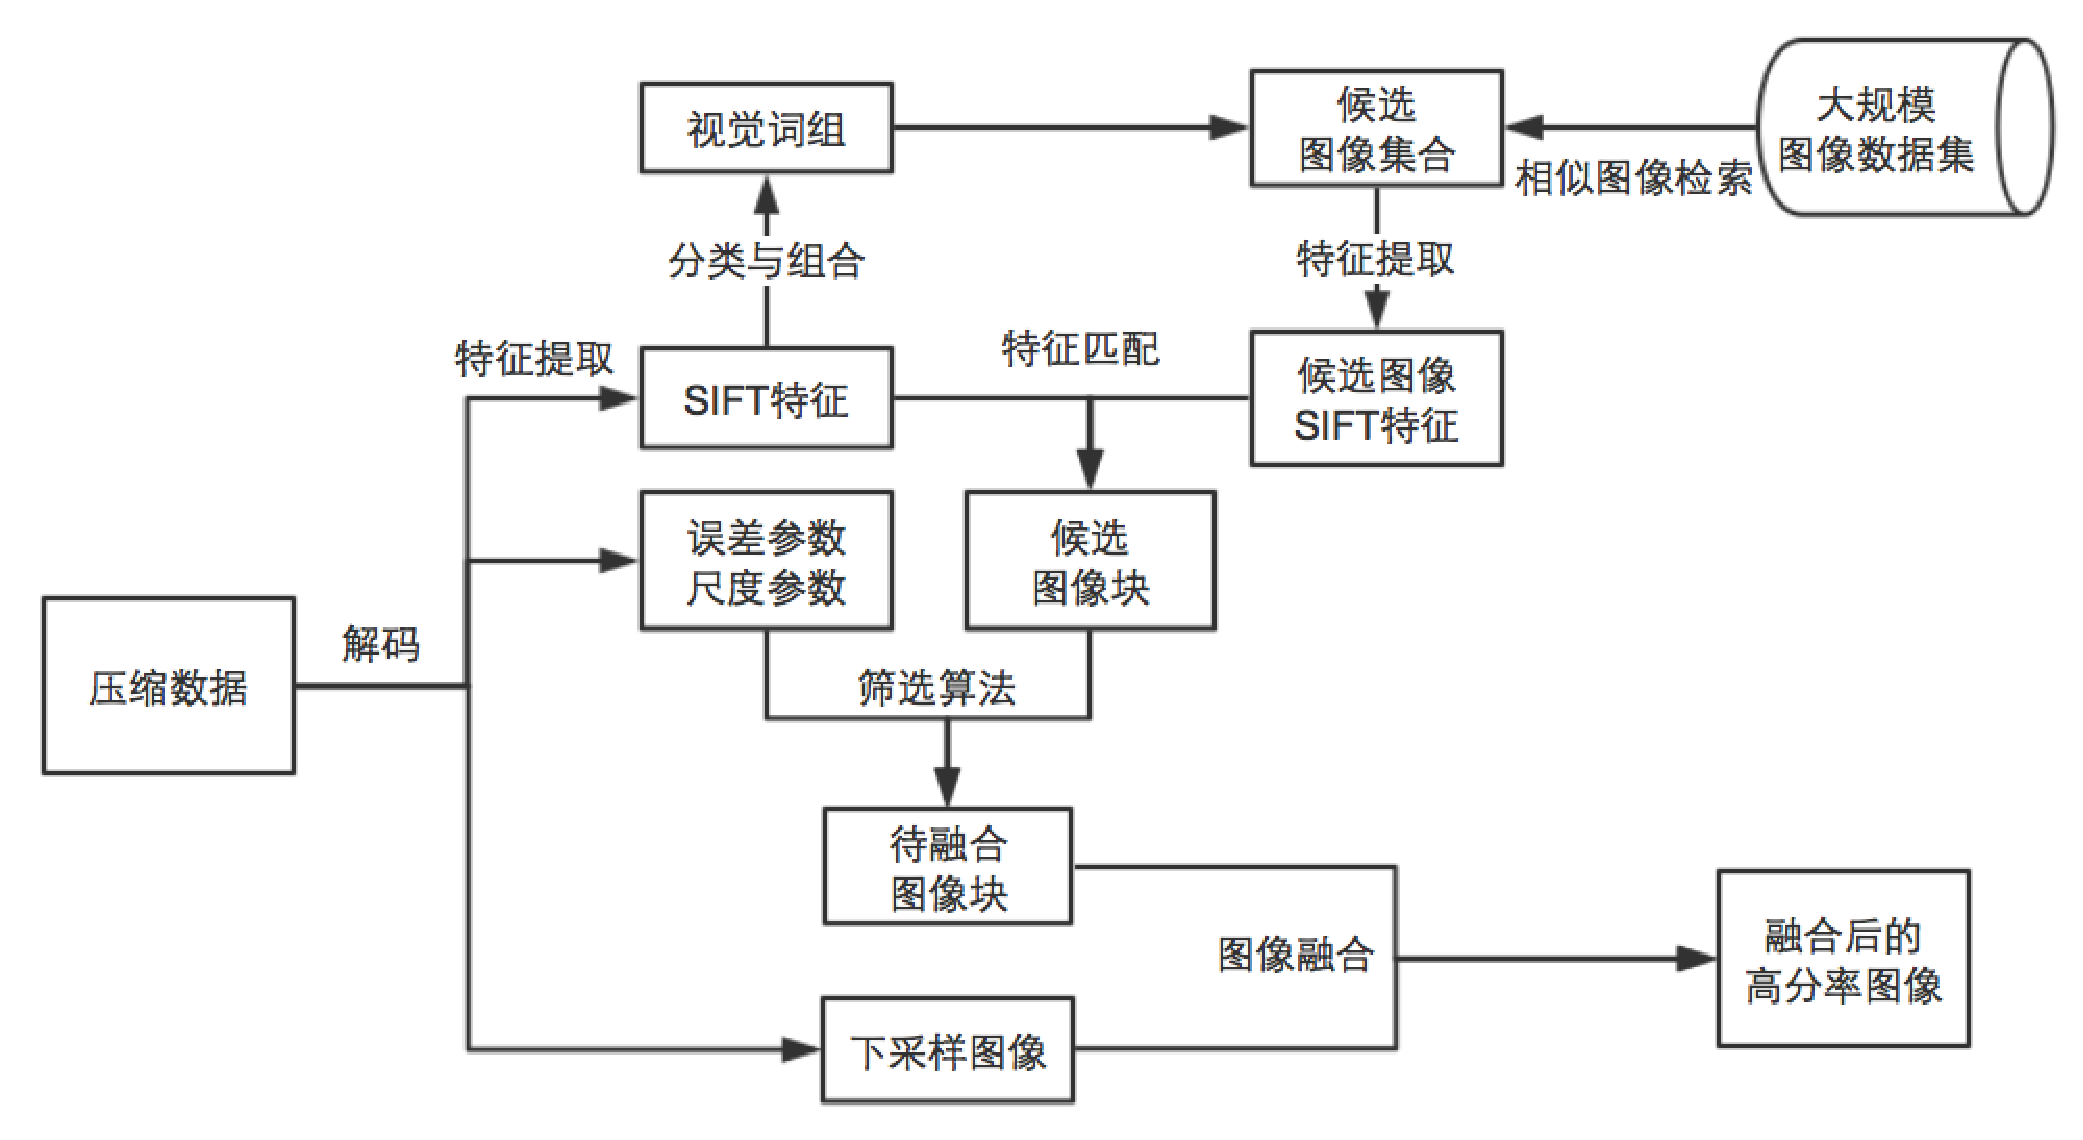
\includegraphics[height=8cm]{serverOnline}
\caption{服务器在线重建流程图}
\label{fig:serverOnline}
\end{figure}


\section{一些格式说明}

\subsection{正文}

\subsubsection{正文字体}

当需要强调某些文字时,建议使用 \verb|\emph{文字}| 命令,也可以直接使用 \verb|\textbf{加粗文字}| 或 \verb|\textit{倾斜文字}| 等。

\subsubsection{脚注}

在正文中插入脚注使用 \verb|\footnote{脚注文本}| 命令\footnote{这里放置脚注的文本内容。}。

\subsubsection{参考文献引用}

在正文中引用参考文献使用序号方式,并根据上下文确定文献引用序号是否采用上标方式。举例:在文献\cite{bib1}中提出一种方法,后续研究对该方法进行了改进\upcite{bib1,bib2}。

\subsection{图形}

本模板提供的文档类 \verb|csoarticle| 本身默认情况下已经包含了 \verb|graphicx| 宏包,因此典型方法是用 \verb|\includegraphics| 命令将图形包含到浮动环境 \verb|figure| 中。图 \ref{fig:sample} 是一个例子。除了 \verb|pdf| 格式外,也支持 \verb|eps|, \verb|jpeg| 等多种格式,具体用法可参看 \verb|graphicx| 宏包的文档。
\begin{figure}
\centering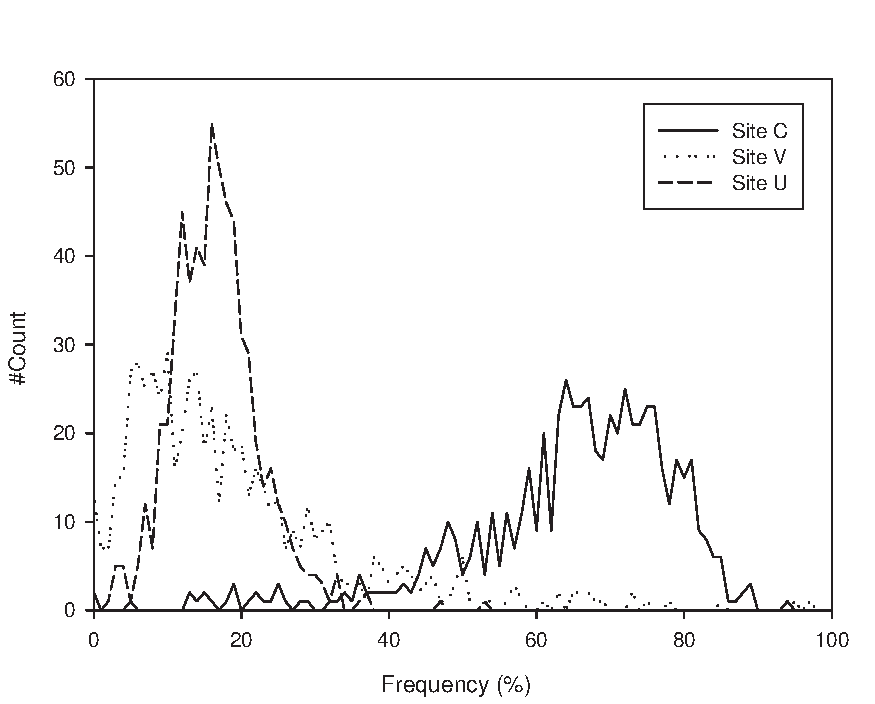
\includegraphics[height=6cm]{figsamp}
\caption{数据曲线图示例}
\label{fig:sample}
\end{figure}

\subsection{表格}

使用浮动环境 \verb|table| 的示例见表\ref{tab:sample}。
\begin{table}
  \caption{表格示例}
  \label{tab:sample}
  \centering
  \begin{tabular}{lcr}%{|l|c|r|}
    \hline
    求解算法                & 系数矩阵的规模    & 执行时间(秒)  \\
    \hline
    Gauss消去法(直接法)     & Mat1903           &  113.27       \\
    Jacobi点迭代            & Mat1784           &  201.36       \\
    \hline
  \end{tabular}
\end{table}


\subsection{参考文献的格式要求}

文献数量应不低于6篇,综述文章文献数量不低于25篇。

注:文中所引的参考文献, 作者均应认真阅读过, 对文献的作者、题目、发表的刊物、年份、卷期号和起止页码等均应核实无误,并按在正文出现的先后顺序编号。标引的序号两边加“[ ]”,作者不超过3人的姓名都写, 超过3人的第三人后面加“,等(et al)” 。无论中外署名,一律姓(大写)先名后,作者姓名之间以逗号分隔。参考文献一律置于文末。文献正文中所有非英文文献需写出对应的英文译文,具体格式要求如下(例子请参看本模板文后的参考文献):
\begin{enumerate}
\item\textbf{期刊:}     作者. 论文题目[J]. 刊名,年,卷(期):起始页码~终止页码.
\item\textbf{专著:}     作者. 书名[M]. 出版地:出版社,出版年.
\item\textbf{译著:}     作者. 书名[M]. 译者. 出版地:出版社,出版年.
\item\textbf{论文集:}   作者. 论文题目[A]. 编者. 文集[C]. 出版地:出版社,出版年. 起始页码~终止页码.
\item\textbf{学位论文:} 作者. 论文题目[D]. 所在城市:保存单位,年份.
\item\textbf{技术标准:} 起草责任者,技术标准代号顺序号—发布年. 技术标准名称[S]. 出版地:出版社,出版年.其中,起草责任者、出版地、出版社、出版年可省。
\item\textbf{专利:}     申请者. 专利名[P]. 国名及专利号,发布日期.
\item\textbf{技术报告:} 作者. 文题[R]. 地名:责任单位,报告代码及编号,年份.
\item\textbf{报纸文章:} 作者. 文题[N]. 报纸名,出版日期(版次).
\item\textbf{在线文献:} 作者. 文题[OL]. [日期]. http://......
\item\textbf{光盘文献:} 作者. 文题[CD]. 出版地:出版者,出版日期.
\item\textbf{其他文献:} 作者. 文题[Z]. 出版地:出版者,出版日期.
\end{enumerate}

\section{结论}

本文给出了………

\section*{致谢(可选)}

应向对论文有帮助的有关人士或单位表示谢意。


%----------------------------------------------------------
% 3. 参考文献
%----------------------------------------------------------

\begin{thebibliography}{2} % 这里的2是指参考文献总数目,需要根据实际情况进行修改
    \bibitem{bib1} H.E.S.Said, T.Tan and K.Baker.Personal identification based on handwriting [J].Pattern Recognition, 33:149-160, Jan. 2000
    \bibitem{bib2} 吴佑寿,丁晓青.汉字识别原理与应用[M],北京:高等教育出版社,1992.8
\end{thebibliography}

\end{document}
